\section[Konstrukce a provoz výzkumných reaktorů]{Konstrukce a provoz výzkumných reaktorů}

Pro pojem "výzkumný reaktor" neexistuje jednotná definice, zahrnuje širokou škálu neenergetických reaktorů, od podkritických souborů přes kritické soubory a reaktory s nízkým výkonem až po výzkumné reaktory s vysokým výkonem.

Rozdělení výzkumných reaktorů také není jasně definované. Například IAEA používá dělení podle výkonu:

\begin{itemize}
    \item Výzkumné reaktory nízkého výkonu do 250~kW,
    \item Výzkumné reaktory středního výkonu od 250~kW do 1~MW,
    \item Výzkumné reaktory vysokého výkonu nad 1~MW.
\end{itemize}

Informace o výzkumných reaktorech lze najít v databázi Research Reactor Database (RRDB), provozované IAEA.

V ČR je podle atomového zákona 263/2016 Sb. výzkumný reaktor definovaný jako:

\begin{quote}
Výzkumným jaderným zařízením se rozumí jaderné zařízení s jaderným reaktorem, které se využívá jako zdroj ionizujícího záření pro účely výzkumu, vzdělávání, výroby radionuklidů, neutronové radiografie, zkoušení materiálů nebo poskytování zdravotních služeb, jejichž odvod tepla nepřesahuje 50~MW a jejichž hlavním účelem není výroba elektřiny nebo tepla.
\end{quote}

\textbf{Podkritický soubor:}

Zařízení, které není schopné udržet štěpnou řetězovou reakci bez externího zdroje neutronů. Jako zdroj neutronů lze použít urychlovače, generátory neutronů nebo radionuklidové zdroje (například $^{252}$Cf). Příklady:

\begin{itemize}
    \item VR-2,
    \item DEPHI (Nizozemsko)
    \item YALINA (Bělorusko).
\end{itemize}

\begin{figure}[H]
    \centering
    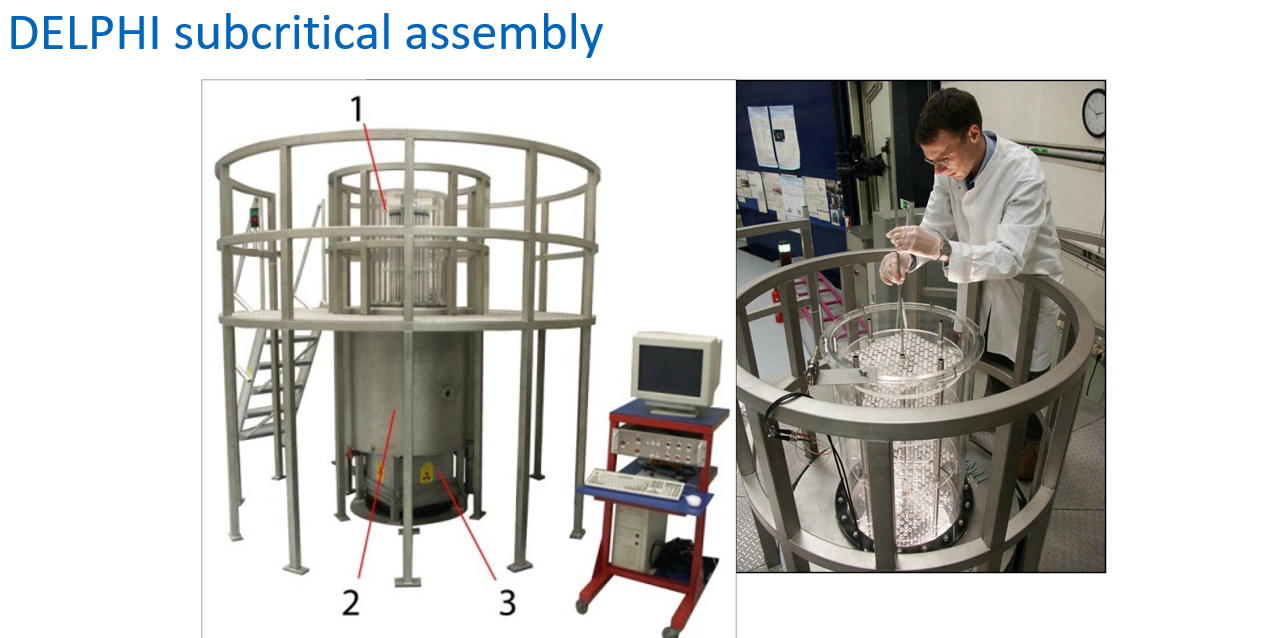
\includegraphics[width=0.75\linewidth]{img/DELPHY_SA.png}
    \caption{DELPHI.}
    \label{fig:enter-label}
\end{figure}

\begin{figure}
    \centering
    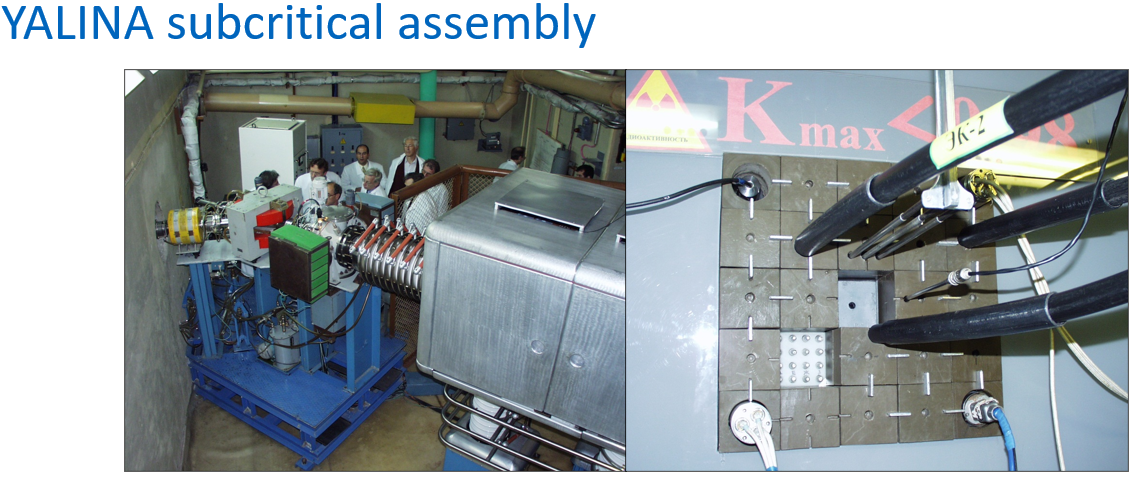
\includegraphics[width=0.75\linewidth]{img/YALINA.png}
    \caption{YALINA.}
    \label{fig:enter-label}
\end{figure}


\textbf{Reaktory nízkého výkonu:}

Určeny především pro výuku a vzdělávání. Existují různé řady reaktorů:

\begin{itemize}
    \item AGN, navrženo Aerojet General Nucleonics (USA),
    \item SUR, navrženo Siemens (Německo),
    \item ARGONAUT, navrženo Argonne National Laboratory (USA),
    \item SLOWPOKE, navrženo Atomic Energy of Canada Limited (Kanada),
    \item TRIGA, navrženo General Atomics (USA): tři modely -- Mark I (bez horizontálních svazků), Mark II (několik horiz. svazků) a Mark III. 
\end{itemize}

\begin{figure}[H]
    \centering
    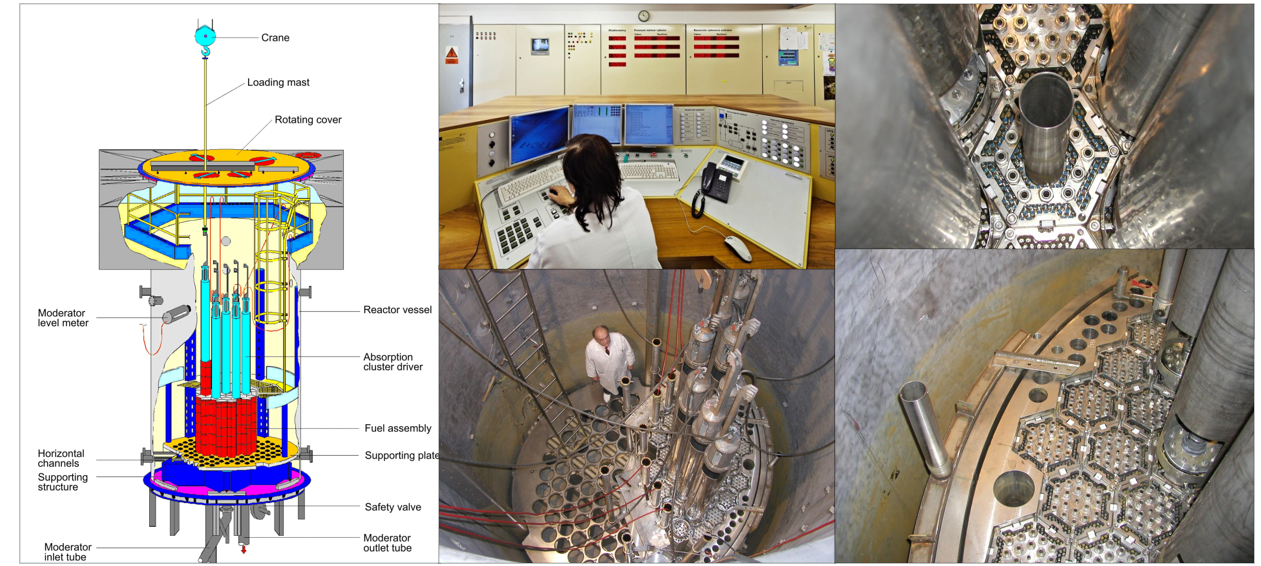
\includegraphics[width=0.75\linewidth]{img/LR0.png}
    \caption{LR0}
    \label{fig:enter-label}
\end{figure}

\textbf{Reaktory středního a vysokého výkonu:}

Žádné typy VR reaktorů středního a vysokého výkonu jako u nízkovýkonových reaktorů (AGN, SUR, ARGONAUT, TRIGA, …). Obvykle použitá unikátní konstrukce a nestaví se více než 2-3 stejné reaktory. Hlavním důvodem unikátní konstrukce VR středního a vysokého výkonu jsou vysoké provozní důvody:

\begin{itemize}
    \item Vysoké počáteční investice,
    \item vysoká spotřeba paliva,
    \item rozsáhlé a drahé přístrojové vybavení,
    \item velký počet zaměstnanců.
\end{itemize}

Efektivní využití reaktoru je nutné pro dlouhodobě udržitelný provoz, to znamená, že reaktory středního nebo vysokého výkonu musí být navrženy pro určité očekávané využití a pro specifické podmínky v zemi/regionu.

Příkladem těchto reaktorů mohou být:

\begin{itemize}
    \item Střední výkon: RA-6 (Argentina, max. 1~MW), HOR (Nizozemsko, max. 2~MW),
    \item Vysoký výkon: FRM II (Německo, max. 20~MW), OPAL (Austrálie, max. 20~MW), LVR-15 (ČR, max. 10~MW).
\end{itemize}

\begin{figure}[H]
    \centering
    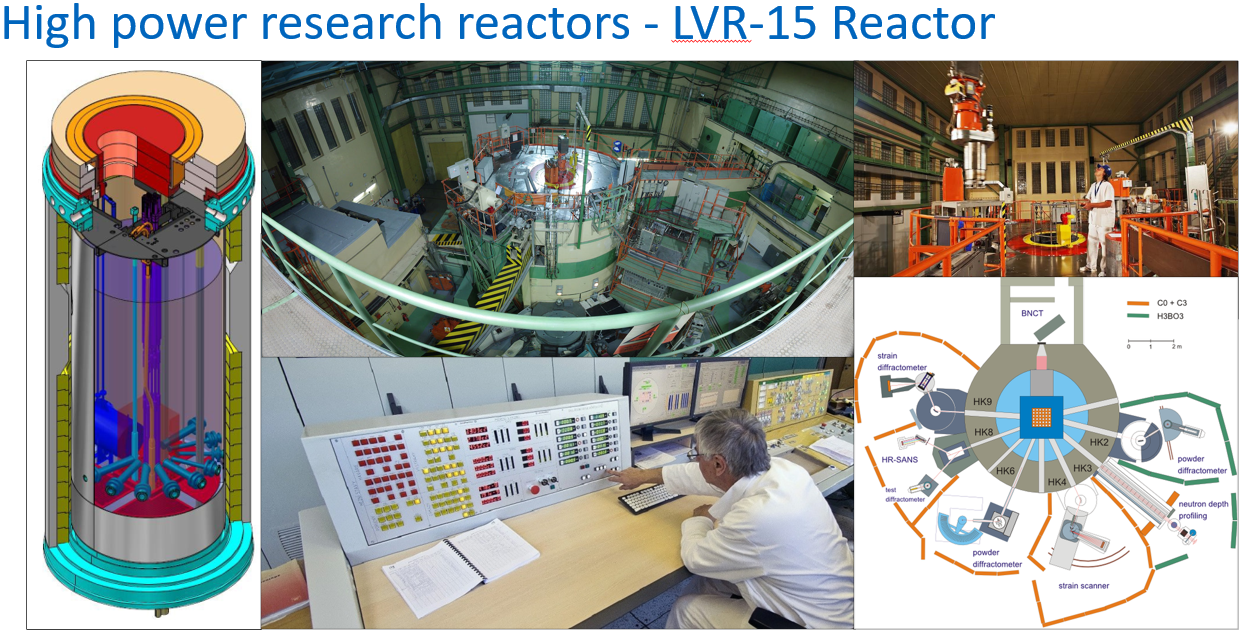
\includegraphics[width=0.75\linewidth]{img/LVR15.png}
    \caption{LVR15}
    \label{fig:enter-label}
\end{figure}

\begin{figure}[H]
    \centering
    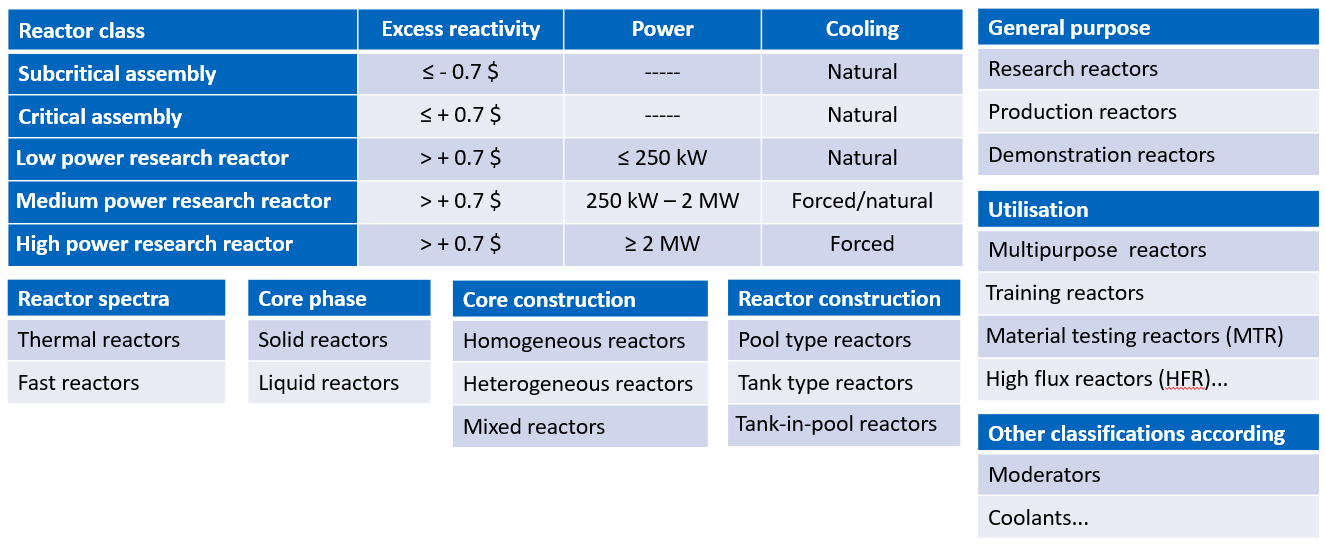
\includegraphics[width=0.75\linewidth]{img/RozděleníRR.png}
    \caption{Rozdělení výzkumných reaktorů.}
    \label{fig:enter-label}
\end{figure}

\subsection{Paliva výzkumných reaktorů}

Co se týče paliv může se jednat o nejrůznější kombinace materiálů, konstrukcí, obohacení, geometrie, forem a stavů. U výzkumných reaktorů není mnoho konstrukčních řad jako u elektráren. Většinou se jedná o unikátní design:

\begin{itemize}
    \item Materiály: $^{235}$U, $^{239}$Pu, $^{233}$U, $^{238}$U, $^{232}$Th,
    \item Obohacení: přírodní, LEU, HEU,
    \item Geometrie: pelety/tyče (EK-10 nebo TRIGA), trubky (VR-1 nebo LVR-15), desky (McMaster nebo OPAL), koule, prstencovité deskové palivo (FRM-II)
    \item Forma: slitina, keramika, kovové,
    \item Stav: pevný, kapalný.
\end{itemize}

Snaha o přechod na nízké obohacení u vše výzkumných reaktorů. Někde se to podařilo, někde to je horší. VR-1 přechod 2005, např FRM-II (Mnichov) má stále HEU.

\begin{figure}[H]
    \centering
    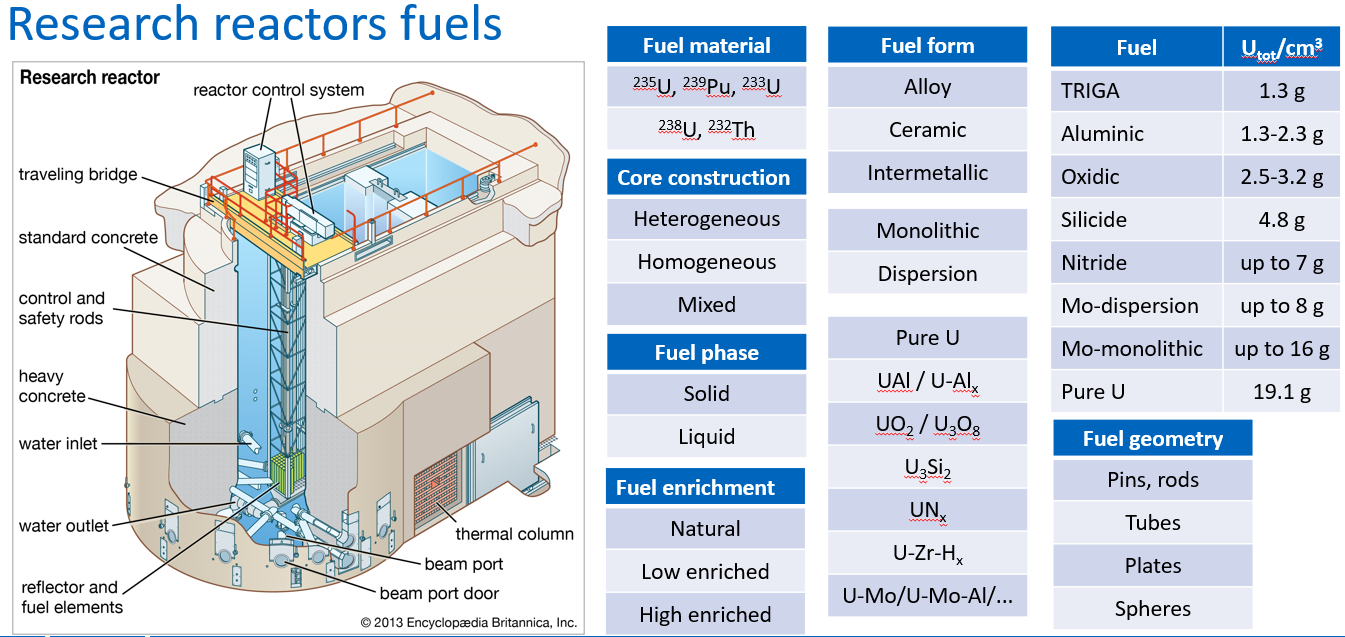
\includegraphics[width=0.75\linewidth]{img/PalivaVýzkumnýchReaktorů.png}
    \caption{Paliva výzkumných reaktorů.}
    \label{fig:enter-label}
\end{figure}

\subsection{Konstrukce výzkumných reaktorů}

Opět co se týče konstrukce může se jednat o nejrůznější kombinace.
Konstrukce -- bazénový typ (VR-1), tankový typ (LVR-15), tank v bazénu (FRM-II)
Základní konstrukční částí výzkumného reaktoru:

\begin{itemize}
    \item Palivo,
    \item moderátor,
    \item chladivo,
    \item reflektor,
    \item absorbátory (tyče),
    \item neutronový zdroj,
    \item experimentální vybavení (in-core /ex-core),
    \item stínění,
    \item řídící systém.
\end{itemize}

Komplexnost jednotlivých systémů závisí na výkonu a komplikovanosti reaktoru.

\textbf{Moderátor} -- voda, těžká voda, grafit, polyethylen
\textbf{Chladivo} -- voda, těžká voda, vzduch, helium
\textbf{Reflektor} -- beryllium, grafit, voda, těžká voda, polyethylen, ocel,
\textbf{Absorbátory} -- bor, kadmium (VR-1), hafnium (OPAL), ocel, europium

\begin{figure}[H]
    \centering
    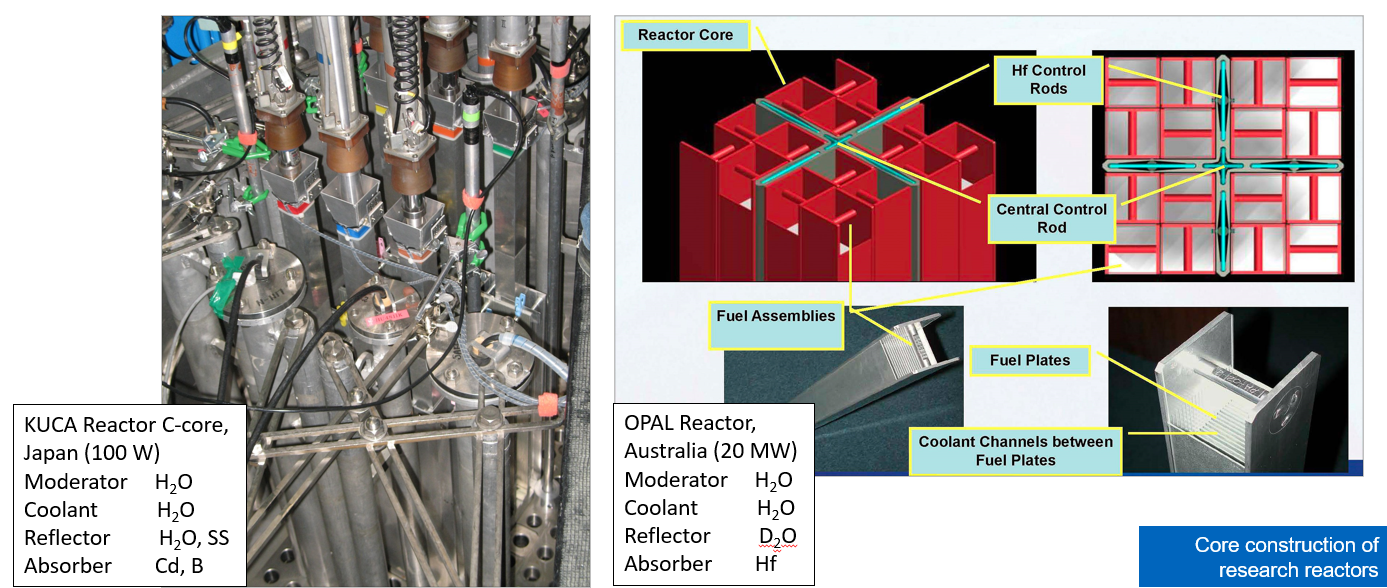
\includegraphics[width=0.75\linewidth]{img/KonfiguraceAZ.png}
    \caption{Konfigurace AZ}
    \label{fig:enter-label}
\end{figure}

\subsection{Experimentální vybavení}

Každý výzkumných reaktor je vybaven různými typy instrumentů pro provádění experimentů, podle toho, k čemu je využíván.  Experimentální vybavení je možné rozdělit podle toho, jestli se nachází přímo v AZ reaktoru nebo vně. \\
Exp. Vybavení v AZ:

\begin{itemize}
    \item Ozařovací pozice -- přímo v AZ, v reflektoru, atd.
    \item Pneumatický systém
    \item Vertikální ozařovací kanály
    \item Smyčky
\end{itemize}

Exp. Vybavení mimo AZ:

\begin{itemize}
    \item Horizontální kanály -- radiální a tangenciální kanály
    \item Zdroj chladných neutronů
    \item Tepelná kolona
    \item Horké komory
\end{itemize}

\subsection{Provoz výzkumných reaktorů}

Provoz výzkumných reaktorů je závislý na jejich výkonu (od miliwattů až po stovky watů) a způsobu využití. Dále závisí, zda se jedná o ustálený provoz nebo provoz v pulzním režimu nebo jestli například dochází k velké valiabilitě provozu (časté změny výkonu, odstavování a spouštění reaktoru). 

Provoz reaktorů nízkého výkonu se většinou liší od provozu reaktorů vysokého výkonu. Reaktory nízkého výkonu jsou často provozovány v denní směnách, zatímco reaktory vysokého výkonu v cyklech, kde provoz probíhá 24/7.

\textbf{Radiační ochrana a bezpečnost:}

Obvykle zanedbatelný nebo malý dopad na životní prostředí a místní obyvatelstvo při běžném provozu, včetně potenciálních havárií. Může mít významný dopad na personál reaktoru při manipulaci s palivem, neutronovými zdroji, ozářenými vzorky nebo při použití experimentálního vybavení.

\textbf{Bezpečnost a ochranná opatření ve výzkumných reaktorech:}

Výzkumné reaktory jsou obvykle velmi odolné vůči radiologické sabotáži. Riziko krádeže jaderného materiálu je značné.
 
\textbf{Jaderná bezpečnost ve výzkumných reaktorech:}

Výzkumné reaktory jsou citlivější z hlediska kritičnosti havárií kvůli zpoždění negativních zpětných účinků při nízké úrovni výkonu (tj. wattech nebo několika kilowattech). Změny výkonu a reaktivity často vyžadují větší pozornost kinetice a dynamice reaktoru. Vliv experimentálního vybavení a vzorků v aktivní zóně a reflektoru může být také velmi důležitý a může významně ovlivnit provoz reaktoru. 

\subsection{Situace ve světě ohledně VR}

\begin{figure}
    \centering
    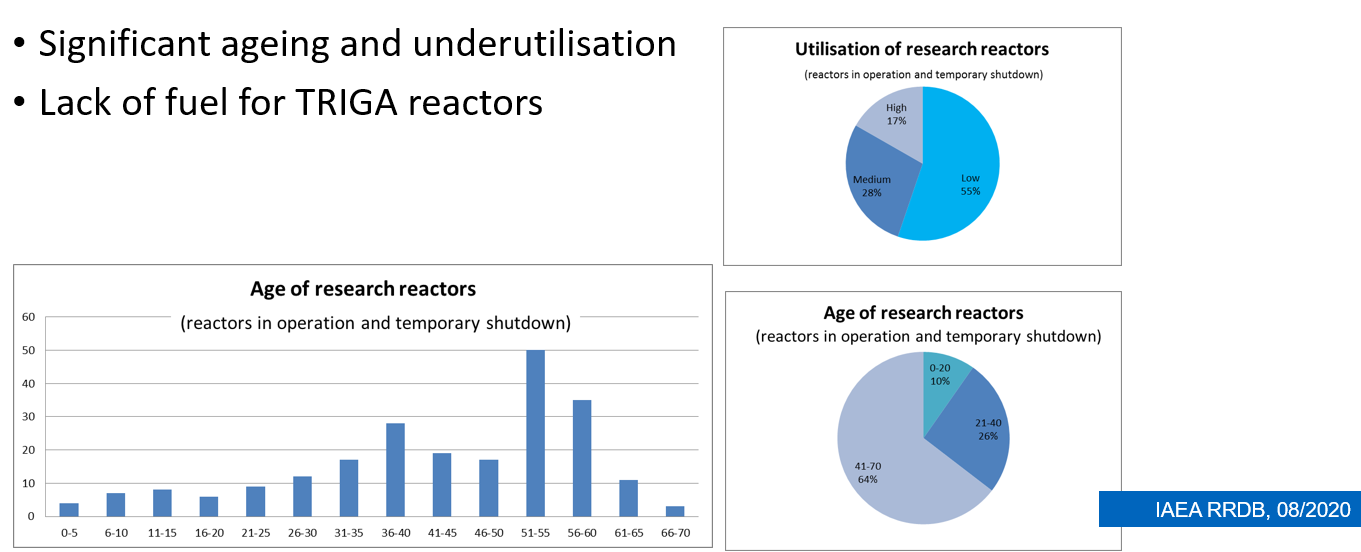
\includegraphics[width=0.75\linewidth]{img/AgeOfRR.png}
    \caption{Situace ohledně VR}
    \label{fig:enter-label}
\end{figure}

V posledních 10--20 letech bylo v USA mnoho výzkumných reaktorů odstaveno a dekomisováno. Podobná situace nastává v Evropě, avšak s přibližně desetiletým zpožděním. Současně jsou však ve světě uvedeny do provozu nebo jsou ve fázi výstavby nové výzkumné reaktory.

Nové výzkumné reaktory v provozu nebo ve fázi uvedení do provozu:

\begin{itemize}
    \item Jordánsko: JRTR reaktor
    \item Ruská federace: PIK reaktor
    \item Čína: CARR reaktor
\end{itemize}

Nové výzkumné reaktory ve výstavbě:

\begin{itemize}
    \item Argentina: RA-10 reaktor, CAREM-25 reaktor (demonstrativní reaktor)
    \item Francie: JHR (Jules Horowitz Reactor)
    \item Saúdská Arábie: LPRR reaktor
    \item Ruská federace: MBIR reaktor, IRV-2M reaktor
    \item Ukrajina: KIPT podkritické zařízení
    \item Tádžikistán: ARGUS FTI homogenní reaktor
    \item Česká republika: VR-2 podkritické zařízení
\end{itemize}

Zatímco některé státy čelí poklesu počtu výzkumných reaktorů, jiné investují do nové generace zařízení, čímž zajišťují pokračující výzkum a vývoj v oblasti jaderné energetiky.
